% Introdução - aprendizado de máquina
A área de aprendizagem de máquina é uma ramificação da grande área de inteligência artificial, dentro da ciência da computação. Essa disciplina tem como objetivo a análise de dados provenientes das mais diversas fontes de modo a realizar inferências sobre tais dados. A tarefa de inferência mais comum é a classificação, onde um método é treinado de forma a capturar características de interesse a partir de padrões existentes nos dados utilizados e, após esse treinamento, é capaz de classificar novos padrões com base no que \emph{aprendeu}. Esse treinamento pode seguir diversos paradigmas, entre eles estão a aprendizagem supervisionada, não-supervisionada e por reforço.

% Paradigmas do aprendizado de máquina
Na aprendizagem supervisionada, os exemplos (ou instâncias) são mostrados ao algoritmo, juntamente com as \emph{respostas} ou classe de cada instância. O treinamento é dito supervisionado pois o classificador tem completo conhecimento das classes da amostra de dados de treino e deve aprender baseado nesta característica. Na abordagem não-supervisionada, o algoritmo recebe as instâncias dos dados sem suas respectivas classes. O objetivo é encontrar padrões em comum entre múltiplas instâncias, criando sua própria categorização (isto é, separação dos dados) interna com base nessas características intrínsecas. O método HMM descrito irá conter algumas instâncias teóricas supervisionadas e não supervisionadas, porém apenas as técnicas supervisionadas serão utilizadas no projeto.


%%%%%%%%%%%%%%%%%%%%%%%%%%%%%%%%%%%%%%%%%%%%%%%%%%%%%%%%%%%%%%%%%%%%%
% Section: Introduction to HMMs
%%%%%%%%%%%%%%%%%%%%%%%%%%%%%%%%%%%%%%%%%%%%%%%%%%%%%%%%%%%%%%%%%%%%%
\subsection{Introduction to HMMs}
\label{sec:introduction.hmms}

% Introdução
Cadeias de Markov são modelos probabilísticos compostos por uma coleção de estados e uma coleção de transições entre esses estados, que correspondem à probabilidade da mudança de um estado para o outro. Os modelos escondidos de Markov seguem esta mesma ideia, porém neles, além da sequência de estados conhecida, existe uma sequência de estados, chamada de caminho (em inglês, \emph{path}), que não é conhecida e cada estado emite símbolos conhecidos (que fazem parte de um alfabeto $ \Sigma $) a partir de uma determinada probabilidade. O objetivo deste modelo é, considerando a sequência de estados conhecida como sendo uma sequência de ``emissões'' de símbolos dentro de um alfabeto específico, determinar qual é a sequência de estados mais provável de ter gerado esta sequência de símbolos.

% Formalização do HMM
Os HMMs são formalizados a seguir. Um modelo escondido de Markov consiste em: (1) um conjunto de estados $ S = \{ S_1, S_2, ..., S_n \} $; (2) uma matriz $ A $ de dimensões $ n $ x $ n $ onde cada célula $ a_{ij} $ dessa matriz representa a probabilidade de se transitar do estado $ i $ para o estado $ j $; (3) uma matriz $ E $ de tamanho $ |\Sigma| $ x $ n $ onde cada entrada $ e_i(b) $ representa a probabilidade de se emitir, no estado $ i $, a entrada observada $ b \in \Sigma $. Esse modelo recebe como entrada uma sequência $ x = x_1 x_2 ... x_L $ de observações e possui uma instância especial $ \pi = \pi_1 \pi_2 ... \pi_L $, onde $ \pi_i \in S $, chamada caminho (ou sequência de estados escondidos), que pode assumir o papel de entrada ou saída do algoritmo dependendo dos objetivos da prova ou modelagem que se deseja obter. A Figura~\ref{gusmao_hmm_structure} sumariza essas definições de forma gráfica. Modelos gráficos deste gênero serão utilizados mais adiante quando soluções para o problema de predição de TFBSs forem propostas.

%\vspace{0.8cm}
%\figuremacroW{gusmao_1_HmmStructureDiscrete}{Esquema de um modelo escondido de Markov}{Neste esquema exemplo, existem 2 estados $S_1$ e $S_2$. Cada um dos dois estados possui transição para si e para o outro estado. A emissão de cada estado, isto é $ e_1(x_i) $ e $ e_2(x_i) $, correspondem a probabilidades pontuais atribuídas a cada possível valor $ x_i $. Observe que a matriz de transição está representada em sua forma vetorial para facilitar a visualização.}{1.0}
%\vspace{0.5cm}

% Figure - HMM structure
\begin{figure}[h!]
\centering
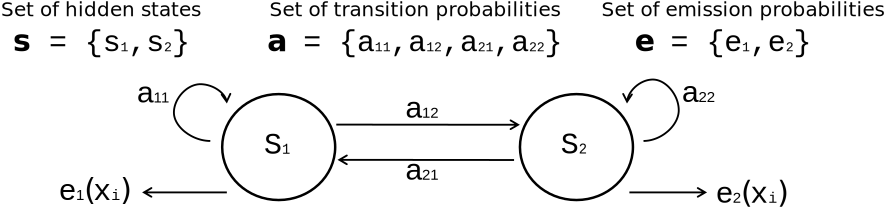
\includegraphics[width=0.99\textwidth]{gusmao_hmm_structure}
\caption[Hidden Markov model scheme]{\textbf{Hidden Markov model scheme.} In this scheme, a simple hidden Markov model is shown. This particular model contains two states: $S_1$ and $S_2$. Each state has a transition probability ($a_{ij}$) to itself and to the other state. The emission probability for each state ($e_i(b)$) corresponds to the discrete probability mass function attributed to each value of a certain input point $x_i$. In this example, the transition and emission matrices are represented as a set of probabilities to facilitate the visualization.}
\label{fig:gusmao_hmm_structure}
\end{figure}

% Equações de transição, emissão e probabilidade conjunta
Realizadas as definições iniciais sobre os parâmetros e entradas do modelo, podemos formalizar de maneira probabilística o conceito de \emph{transição} e \emph{emissão}, respectivamente, segundo as Equações~\ref{eq:hmm1} e~\ref{eq:hmm2}. Tais definições correspondem à base de todos os resultados subsequentes e devem ser entendidos como cláusulas básicas para a teoria dos HMMs.

\begin{equation}\label{eq:hmm1}
    a_{kl} = P(\pi_i = l | \pi_{i-1} = k)
\end{equation}

\begin{equation}\label{eq:hmm2}
    e_k(b) = P(x_i = b | \pi_i = k)
\end{equation}

% Propriedade chave dos HMM
Além das ações básicas de transição e emissão, a teoria dos HMMs possui uma propriedade chave: a probabilidade de prosseguir do estado $ i $ para o estado $ i+1 $ depende apenas da probabilidade no estado $ i $. Dessa forma, o processo estocástico faz com que as probabilidades sejam sumarizadas em cada estado, de forma indutiva. Podemos generalizar a propriedade chave como: a probabilidade de prosseguir do estado $ i $ para o estado $ i+1 $ depende apenas da probabilidade dos $ T $ estados anteriores, definindo um HMM de ordem $ T $. Utilizando um estado auxiliar inicial $ 0 $, no qual o modelo se encontra no início do processo, e um estado auxiliar final $ L + 1 $ (também denotado posteriormente como $ \epsilon $), no qual o modelo se encontra no fim do processo, podemos representar esse conceito chave, para o caso de ordem 1, segundo a Equação~\ref{eq:hmm3}.

\begin{equation}\label{eq:hmm3}
    P(x,\pi) = a_{0\pi_1} \prod_{i=1}^{L} e_{\pi_i}(x_i)a_{{\pi_i}{\pi_{i+1}}}
\end{equation}

% HMMs contínuos
Podemos definir as emissões como discretas ou contínuas. A diferença não irá afetar a modelagem teórica a seguir, pelo fato de que: no caso discreto, basta que as probabilidades (denotadas por $ P(\cdot) $) sejam funções (massa) de probabilidade; em contrapartida, no caso contínuo, as probabilidades $ P(\cdot) $ seriam funções densidade de probabilidade. Os sinais utilizados neste projeto são de natureza contínua, portanto as emissões irão corresponder a distribuições gaussianas (Equação~\ref{eq:gaussiana}). Isto significa que cada emissão, em cada estado, será representada através dos parâmetros de uma função densidade de probabilidade do tipo normal: a média $ \mu $ e o desvio padrão $ \sigma $.

\begin{equation}\label{eq:gaussiana}
    f(x;\mu,\sigma) = \frac{1}{\sqrt{2\pi\sigma^2}} {e}^{-\frac{{(x-\mu)}^2}{2\sigma^2}}, -\infty < x < \infty, \sigma > 0
\end{equation}

% HMMs multivariados
Além de contínuos, os modelos escondidos de Markov podem ser multivariados. Novamente, o formalismo a seguir se modificará apenas no que concerne à adição de dimensões. No modelo, a única diferença seria que a matriz de emissões $ E $ teria uma dimensão adicional de tamanho $ d $, onde $ d $ é a dimensionalidade do modelo (isto é, a quantidade de sinais que serão simultaneamente inseridos). A entrada $ e_{ij}(b) $ desta matriz com três dimensões representaria a emissão para o $i-$ésimo estado, para o $j-$ésimo sinal, para um valor observado $ b $.

% A seguir: predição e estimação
Os algoritmos apresentados na Seção~\ref{sec:hmmpredicao} consistem em métodos para se descobrir o caminho $ \pi $ a partir de uma sequência de caracteres $ x $ utilizando um modelo com os parâmetros $ A $ e $ E $ definidos. Nesses métodos a Equação~\ref{eq:hmm3} será explorada e serão criadas novas variáveis para ajudar no entendimento. Os algoritmos apresentados na Seção~\ref{sec:hmmestimacao} mostram formas de se estimar os parâmetros $ A $ e $ E $ para um modelo de Markov escondido, de forma supervisionada ou não supervisionada.

%%%%%%%%%%%%%%%%%%%%%%%%%%%%%%%%%%%%%%%%%%%%%%%%%%%%%%%%%%%%%%%%%%%%%
% Section: Decoding Methods
%%%%%%%%%%%%%%%%%%%%%%%%%%%%%%%%%%%%%%%%%%%%%%%%%%%%%%%%%%%%%%%%%%%%%
\subsection{HMM Decoding Methods}
\label{sec:hmm.decoding.methods}

% Introdução - intuição 1
Dado o formalismo definido na Seção~\ref{sec:hmmintro}, existem, basicamente, três problemas que devem ser resolvidos para que o modelo tenha aplicações práticas:

\begin{center}
  \begin{tabular}{lp{.8\linewidth}}
    {\bf Problema 1} & Dada a sequência observada $ x = x_1 x_2 ... x_L $ e um modelo composto por $ \theta = \{A,E\} $, como é escolhida a sequência $ \pi = \pi_1 \pi_2 ... \pi_L $ que é ótima dado algum critério significativo (isto é, que melhor explica as observações)? \\[0.2cm]
    {\bf Problema 2} & Dada a sequência observada $ x = x_1 x_2 ... x_L $ e um modelo composto por $ \theta = \{A,E\} $, como é computada $ P(x|\theta) $, isto é, a probabilidade da sequência observada, dado o modelo? \\[0.2cm]
    {\bf Problema 3} & Como os parâmetros $ \theta = \{A,E\} $ podem ser ajustados de forma a maximizar $ P(x|\theta) $? \\[0.2cm]
  \end{tabular}
\end{center}

% Introdução - intuição 2
O primeiro problema proposto, que aborda a parte \emph{escondida} do HMM, será abordado na Seção~\ref{ssec:viterbi}, ao definir o método de Viterbi. O segundo problema será utilizado para avaliar a probabilidade posterior na Seção~\ref{ssec:probposterior} (correspondente, mais especificamente, aos métodos \emph{forward} ou \emph{backward}). E finalmente, o terceiro problema, diretamente solucionado através do simples método da verossimilhança na Seção~\ref{sec:hmmestimacao}, faz com que sejamos capazes de treinar o modelo.

% Introdução - predição
Nesta seção serão definidos os dois principais métodos para se predizer sequências de estados escondidos $ \pi $ a partir de um HMM e de entradas (sequências de símbolos $ x $). O primeiro método segue diretamente das definições anteriores, a partir da utilização do paradigma de programação dinâmica para resolver o problema da exaustão inicial. O segundo método resulta em um vetor de probabilidades posterior de tamanho igual ao número de estados, para cada elemento do vetor de entrada. Neste método, que geralmente produz predições mais acuradas que o primeiro, o caminho $ \pi $ pode ser avaliada de várias formas, incluindo a aceitação do estado que possui a maior probabilidade posterior para cada posição da sequência de entrada.

%%%%%%%%%%%%%%%%%%%%%%%%%%%%%%%%%%%%%%%%%%%%%%%%%%%%%%%%%%%%%%%%%%%%%
% Section: Viterbi Algorithm
%%%%%%%%%%%%%%%%%%%%%%%%%%%%%%%%%%%%%%%%%%%%%%%%%%%%%%%%%%%%%%%%%%%%%
\subsubsection{Viterbi Algorithm}
\label{sec:viterbi.algorithm}

% Introdução - decodificação
Ao introduzir uma sequência de estados escondidos $ \pi $ no modelo, se torna impossível descrever deterministicamente em qual estado do modelo estamos apenas através da observação do símbolo correspondente da sequência de entrada $ x $. Encontrar o significado da sequência de entrada em termos da sequência de estados escondidos se chama decodificação, no jargão original de reconhecimento de padrões sonoros.

% Introdução - viterbi
O Algoritmo de Viterbi foi proposto por Andrew Viterbi, em 1976, como um algoritmo de decodificação para códigos convolucionais sobre conexões digitais de comunicação que continham alto nível de ruído. Após sua proposição, esse algoritmo foi aplicado em áreas como celulares digitais CDMA e GSM, modems discados, satélites, comunicações espaciais, redes sem fio 802.11 e atualmente, é bastante utilizado em reconhecimento de fala, linguística computacional e bioinformática.

% Definição formal
O Algoritmo de Viterbi pertence ao paradigma da programação dinâmica e consiste em descobrir qual é o caminho mais provável $ \pi^\ast $ dada a sequência de emissão $ x $. A Equação~\ref{eq:hmm4} descreve em termos formais essa proposição.

\begin{equation}\label{eq:hmm4}
    \pi^\ast = {argmax}_\pi P(x,\pi)
\end{equation}

% Algoritmo - intro
A forma exaustiva de resolução de tal algoritmo seria calcular as probabilidades $ P(x,\pi) $ para todas as sequências $ \pi $ existentes. Entretanto, conforme aumentamos o tamanho $ L $ da sequência de entrada, o número total de combinações de estados que constituem as sequências $ \pi $ cresce exponencialmente, e quanto maior o número de estados, mais agressivo é tal crescimento. Felizmente, Viterbi apontou uma solução baseada em programação dinâmica, onde o caminho mais provável $ \pi^\ast $ pode ser encontrado recursivamente.

% Algoritmo - variável de viterbi
Suponha que criemos variáveis de Viterbi $ v_k(i) $, que correspondem à probabilidade do caminho mais provável do prefixo $ x_1 ... x_i $ que termina no estado $ S_k $. Supondo que tais probabilidades são conhecidas para o todos os estados $ k $ podemos calcular essas probabilidades para o prefixo $ x_1 ... x_{i+1} $ como descrito na Equação~\ref{eq:vvit}.

\begin{equation}\label{eq:vvit}
    v_l(i+1) = e_l(x_{i+1}) {max}_k(v_k(i) a_{kl})
\end{equation}

% Algoritmo - viterbi
Dado que todas as sequências se iniciam em um estado inicial $ 0 $, podemos definir as variáveis de Viterbi para este estado inicial como $ v_0(0) = 1 $ e $  v_k(0) = 0 $ para todos os outros estados que não o inicial. A partir destas variáveis iniciais, podemos continuar calculando as variáveis dos próximos estados segundo a Equação~\ref{eq:vvit} e manter um ponteiro $ ptr $ para os estados que possuíram a maior probabilidade em cada iteração. Tal algoritmo, que é possível dada a propriedade chave das cadeias de Markov, é definido a seguir:

\begin{center}
  \begin{spacing}{1.0}
    \begin{tabular}{l}
      \hline \\[-0.25cm]
      \hspace{1.2cm} {\large {\bf \emph{ Algoritmo de Viterbi } } } \hspace{1.2cm} \\[0.1cm]
      \hline \\[-0.25cm]
      \hspace{0.2cm} {\bf 1. Inicialização:} \\
      \hspace{0.9cm} 1.1. $ v_0(0) = 1 $ \\
      \hspace{0.9cm} 1.2. $ v_k(0) = 0 $ para $ k > 0 $ \\
      \hspace{0.2cm} {\bf 2. Recursão $ (i = 1, ..., L) $:} \\
      \hspace{0.9cm} 2.1. $ v_l(i) = e_l(x_i) {max}_k(v_k(i-1)a_{kl}) $ \\
      \hspace{0.9cm} 2.2. $ {ptr}_i(l) = {argmax}_k(v_k(i-1)a_{kl}) $ \\
      \hspace{0.2cm} {\bf 3. Terminação:} \\
      \hspace{0.9cm} 3.1. $ P(x,\pi^\ast) = {max}_k(v_k(L)a_{k\epsilon}) $ \\
      \hspace{0.9cm} 3.2. $ \pi_{L}^{\ast} = {argmax}_k(v_k(L)a_{k\epsilon}) $ \\
      \hspace{0.2cm} {\bf 4. Remontagem $ (i = L, ..., 1) $:} \\
      \hspace{0.9cm} 4.1. $ \pi_{i-1}^{\ast} = {ptr}_i(\pi_{i}^{\ast}) $ \\[0.1cm]
      \hline
    \end{tabular}
  \end{spacing}
\end{center}

% Problemas operacionais
Existem alguns problemas práticos de implementação em relação ao Algoritmo de Viterbi. O mais severo decorre do fato de que multiplicar diversas probabilidades baixas irá gerar números de ordens extremamente baixas, o que ocasiona em erros de estouro negativo (\emph{underflow}) quando não tratado de forma correta. A solução mais utilizada consiste em realizar o algoritmo no espaço logarítmico, o que faria com que todas as multiplicações virassem somatórios. Esse tipo de detalhe foge ao escopo deste trabalho e não será abordado.

%%%%%%%%%%%%%%%%%%%%%%%%%%%%%%%%%%%%%%%%%%%%%%%%%%%%%%%%%%%%%%%%%%%%%
% Section: Posterior Probability
%%%%%%%%%%%%%%%%%%%%%%%%%%%%%%%%%%%%%%%%%%%%%%%%%%%%%%%%%%%%%%%%%%%%%
\subsubsection{Posterior Probability}
\label{ssec:posterior.probability}

% Introdução - probabilidade posterior
Além do Algoritmo de Viterbi, podemos realizar a decodificação através do cálculo da probabilidade posterior de estar em cada estado escondido, em cada posição da sequência de entrada. Extrair o conjunto mais provável de estados escondidos desta abordagem pode ser realizado de forma simples como observar qual estado possui a maior probabilidade posterior para cada posição da sequência, ou de formas mais complexas como fixar um ponto de corte para aceitação de estados escondidos baseado nestas probabilidades. Além de permitir a extração do conjunto mais provável de estados de uma forma mais elaborada, o cálculo das probabilidades posteriores permite que seja visualizada a forma como as transições estão ocorrendo. Por essas razões, geralmente esta abordagem é preferível em relação ao Algoritmo de Viterbi.

% Probabilidade posterior de Bayes
A probabilidade posterior pode ser definida mais formalmente como como sendo a probabilidade de, em uma certa posição da cadeia de caracteres, observarmos o estado escondido  $ k $, dada a sequência observada. Pelo teorema de Bayes, é possível colocar essa proposição em termos matemáticos (Equação~\ref{eq:hmm5}).

\begin{equation}\label{eq:hmm5}
    P(\pi_i = k | x) = \frac{P(x, \pi_i = k)}{P(x)}
\end{equation}

% Probabilidade de evidência
Primeiramente, será focado o cálculo da cláusula $ P(x) $, isto é, a evidência de uma certa cadeia de caracteres $ x $ dentro de todas as possibilidades de cadeias de tamanho $ L $. Formalmente, isso pode ser definido em relação ao caminho segundo a Equação~\ref{eq:hmm6}.

\begin{equation}\label{eq:hmm6}
    P(x) = \sum_{\pi} P(x,\pi)
\end{equation}

% Variável forward
O cálculo exaustivo da Equação~\ref{eq:hmm6} é impossível pois o número de caminhos cresce exponencialmente com o tamanho da sequência (conforme já foi visto no contexto de Viterbi). Porém podemos avaliar esta expressão com a mesma ideia de Viterbi mostrada, apenas modificando os passos de maximização por somatórios. Neste novo algoritmo a variável $ f_k(i) $, chamada variável \emph{forward}, é utilizada assim como a variável de Viterbi (Equação~\ref{eq:hmm7}). A variável \emph{forward} corresponde à probabilidade de observar a sequência $ x $ até (e incluindo) $ x_i $ de tal forma que $ \pi_i = k $. A recursão utilizada pelo algoritmo é definida na Equação~\ref{eq:fvar}.

\begin{equation}\label{eq:hmm7}
    f_k(i) = P(x_1 ... x_i, \pi_i = k)
\end{equation}

\begin{equation}\label{eq:fvar}
    f_l(i+1) = e_l(x_{i+1}) \sum_{k}{f_k(i) a_{kl}}
\end{equation}

% Algoritmo forward
O algoritmo é mostrado a seguir. Assim como o Algoritmo de Viterbi, este método está sujeito a estouros negativos. Tal problema não pode ser resolvido da mesma forma como a Equação~\ref{eq:hmm4} foi por conter somatórios em sua própria natureza. A solução está novamente em se trabalhar em um espaço logarítmico, porém utilizando abordagens mais complexas.

\begin{center}
  \begin{spacing}{1.0}
    \begin{tabular}{l}
      \hline \\[-0.25cm]
      \hspace{1.3cm} {\large {\bf \emph{ Algoritmo Forward } } } \hspace{1.3cm} \\[0.1cm]
      \hline \\[-0.25cm]
      \hspace{0.2cm} {\bf 1. Inicialização:} \\
      \hspace{0.9cm} 1.1. $ f_0(0) = 1 $ \\
      \hspace{0.9cm} 1.2. $ f_k(0) = 0 $ para $ k > 0 $ \\
      \hspace{0.2cm} {\bf 2. Recursão $ (i = 1, ..., L) $:} \\
      \hspace{0.9cm} 2.1. $ f_l(i) = e_l(x_i) \sum_{k}{f_k(i-1) a_{kl}} $ \\
      \hspace{0.2cm} {\bf 3. Terminação:} \\
      \hspace{0.9cm} 3.1. $ P(x) = \sum_{k}{f_k(L) a_{k\epsilon}} $ \\[0.1cm]
      \hline
    \end{tabular}
  \end{spacing}
\end{center}

% Explorando Bayes
Continuando a busca pela probabilidade posterior, podemos explorar o termo $ P(x, \pi_i = k) $. Ao aplicar a propriedade chave dos modelos de Markov, podemos realizar a decomposição demonstrada na Equação~\ref{eq:hmm8}. A segunda linha desta equação ocorre porque tudo que ocorre depois do estado $ k $ depende apenas do que ocorre no estado $ k $.

\begin{equation}\label{eq:hmm8}
    \begin{array}{lcl} 
        P(x, \pi_i = k) & = & P(x_1 ... x_i, \pi_i = k) P(x_{i+1} ... x_L | x_1 ... x_i, \pi_i = k) \\ 
                        & = & P(x_1 ... x_i, \pi_i = k) P(x_{i+1} ... x_L | \pi_i = k)
    \end{array}
\end{equation}

% Variável backward
É bastante claro que o primeiro termo da segunda linha da Equação~\ref{eq:hmm8} corresponde à variável \emph{forward} $ f_k(i) $ cujo cálculo foi apresentado anteriormente. Para calcular a probabilidade posterior precisamos apenas abordar o segundo termo da segunda linha da Equação~\ref{eq:hmm8}. É possível, então, criar outra variável, chamada \emph{backward}, para calcular o termo restante. Obviamente, essa variável é definida como na Equação~\ref{eq:hmm9}.

\begin{equation}\label{eq:hmm9}
    b_k(i) = P(x_{i+1} ... x_L | \pi_i = k)
\end{equation}

% Algoritmo backward
Para calcular tais variáveis é mostrado o Algoritmo \emph{backward} a seguir. Tal algoritmo é análogo ao \emph{forward} porém ao invés de proceder do início da sequência até o ponto desejado, ele procede do fim da sequência até o ponto desejado.

\begin{center}
  \begin{spacing}{1.0}
    \begin{tabular}{l}
      \hline \\[-0.25cm]
      \hspace{1.3cm} {\large {\bf \emph{ Algoritmo Backward } } } \hspace{1.3cm} \\[0.1cm]
      \hline \\[-0.25cm]
      \hspace{0.2cm} {\bf 1. Inicialização:} \\
      \hspace{0.9cm} 1.1. $ b_k(L) = a_{k\epsilon}, \forall k $ \\
      \hspace{0.2cm} {\bf 2. Recursão $ (i = L-1, ..., 1) $:} \\
      \hspace{0.9cm} 2.1. $ b_k(i) = \sum_{l}{a_{kl} e_l(x_{i+1}) b_l(i+1)} $ \\
      \hspace{0.2cm} {\bf 3. Terminação:} \\
      \hspace{0.9cm} 3.1. $ P(x) = \sum_{l}{a_{0l} e_l(x_1) b_l(1)} $ \\[0.1cm]
      \hline
    \end{tabular}
  \end{spacing}
\end{center}

% Probabilidade posterior
A partir dos Algoritmos \emph{forward} e \emph{backward} podemos calcular a probabilidade posterior conforme definida na Equação~\ref{eq:hmm5} através de uma simples substituição dos termos nesta equação pelas respectivas variáveis criadas (Equação~\ref{eq:hmm10}). O termo $ P(x) $ nesta equação pode ser calculado através da aplicação de um dos algoritmos, \emph{forward} ou \emph{backward} na sequência inteira.

\begin{equation}\label{eq:hmm10}
    P(\pi_i = k | x) = \frac{f_k(i) b_k(i)}{P(x)} 
\end{equation}

%%%%%%%%%%%%%%%%%%%%%%%%%%%%%%%%%%%%%%%%%%%%%%%%%%%%%%%%%%%%%%%%%%%%%
% Section: HMM Parameter Estimation
%%%%%%%%%%%%%%%%%%%%%%%%%%%%%%%%%%%%%%%%%%%%%%%%%%%%%%%%%%%%%%%%%%%%%
\subsection{HMM Parameter Estimation}
\label{sec:hmm.parameter.estimation}

% Introdução - estimação
Na Seção~\ref{sec:hmmpredicao}, algoritmos para determinar a sequência de estados escondidos foram definidos. Nesta seção, será demonstrado um método para a criação de tais HMMs, isto é, a estimação dos parâmetros que compõem o HMM (a matriz de transições $ A $ e o vetor de emissões $ E $). A técnica escolhida, máxima verossimilhança, consiste na estimação mais simples possível. A ideia é que os parâmetros sejam o mais próximo possível dos observados nos dados de treinamento. Esta abordagem é, portanto, supervisionada. Caso fosse necessária a estimação de parâmetros um HMM sem informações de classe a priori, um método não-supervisionado como o Baum-Welch teria que ser utilizado. Neste método, estimações são feitas através de aproximações baseadas no algoritmo de Maximização da Esperança (EM, em Inglês \emph{Expectation Maximization}).

% Modelo - arte
Como mencionado, podemos estimar os parâmetros de forma supervisionada ou não supervisionada. Entretanto, o modelo geral, isto é, a sequência de estados $ S $, já deverá estar corretamente modelada. A criação de um modelo oscila bastante entre os que acreditam nesta tarefa como uma arte e naqueles que desenvolvem métodos específicos, geralmente baseados em duração probabilística dos estados. De qualquer forma, tal tarefa não será mencionada. Os modelos originais desenvolvidos neste trabalho foram idealizados com base nos padrões dos dados e sua robustez foi aferida de forma puramente empírica.

% Introdução - máxima verossimilhança
O método da máxima verossimilhança é a forma mais simples de se estimar os parâmetros $ A $ e $ E $ dos modelos escondidos de Markov. Neste tipo de estimação, é utilizada uma sequência de símbolos $ x $ com sequência de estados conhecida $ \pi $ para calcular os parâmetros mais verossímeis.

% Método - máxima verossimilhança
Para o caso discreto, de forma intuitiva, será realizada a simples contagem do número de vezes em que acontece cada evento relacionado aos parâmetros. Denotando por $ A_{kl} $ o número de ocorrências de transições entre os estados $ k $ e $ l $ (não confundir com $ a_{kl} $, que é a probabilidade desta transição), e $ E_k(b) $ o número de emissões do símbolo $ b $ no estado $ k $, o estimador de máxima verossimilhança consiste na simples aplicação das Equações~\ref{eq:hmm11} e~\ref{eq:hmm12}.

\begin{equation}\label{eq:hmm11}
    a_{kl} = \frac{A_{kl}}{\sum_{l^\prime} A_{k{l}^{\prime}}}
\end{equation}

\begin{equation}\label{eq:hmm12}
    e_k(b) = \frac{E_k(b)}{\sum_{b^\prime} E_k(b^\prime)}
\end{equation}

% Método - máxima verossimlhança contínuo
Generalizando para o caso contínuo, tem-se uma função de densidade $ p(x|\Theta) $ governada pelo conjunto de parâmetros $ \Theta $. No caso de uma gaussiana, por exemplo, $ \Theta $ corresponde às médias e desvios padrões das entradas utilizadas. Suponha que tenhamos também um conjunto de dados de tamanho $ T $ obtido a partir desta distribuição, isto é, $ X = \{X_1,...,X_T\} $. A densidade resultante das amostras é dada pela Equação~\ref{eq:hmm13}.

\begin{equation}\label{eq:hmm13}
    p(X|\Theta) = \prod_{i=1}^{T}{ p(X_i|\Theta) } = L(\Theta|X)
\end{equation}

% Método - máxima verossimlhança contínuo
Essa função $ L(\Theta|X) $ é chamada de verossimilhança dos parâmetros dado o conjunto de entradas $ X $. De forma intuitiva, ela pode ser pensada como uma função dos parâmetros $ \Theta $ onde o conjunto de dados $ X $ se encontra fixo. No problema da máxima verossimilhança, o objetivo é encontrar o conjunto de parâmetros $ \Theta $ que maximize a função $ L $ (Equação~\ref{eq:hmm14}).

\begin{equation}\label{eq:hmm14}
    {\Theta}^{\ast} = {{argmax}}_{\Theta}{L(\Theta|X)}
\end{equation}

% Método - máxima verossimlhança contínuo
Esse problema pode ser facilmente resolvido para o caso da gaussiana (onde $ \Theta = \{\mu,\sigma\} $), bastando igualar a derivada de $ log(L(\Theta|X)) $ a zero e resolver diretamente para $ \mu $ e $ \sigma $. O motivo para o uso da função $ log $ é que ela torna o problema analiticamente mais fácil. Para outras distribuições, entretanto, técnicas mais elaboradas são necessárias, dado que a solução para as expressões analíticas não podem ser encontradas diretamente. Tais detalhes não serão expostos, visto que neste projeto serão utilizadas apenas gaussianas para representar os sinais de entrada.
